\setcounter{equation}{0} \numberwithin{equation}{section}

\section{Thoreau}
You never gain something but that you lose something.\\
		-- Thoreau
\section{Unknown}
And dropping a barbell he points to the sky\\

\begin{figure}[h]
\centering
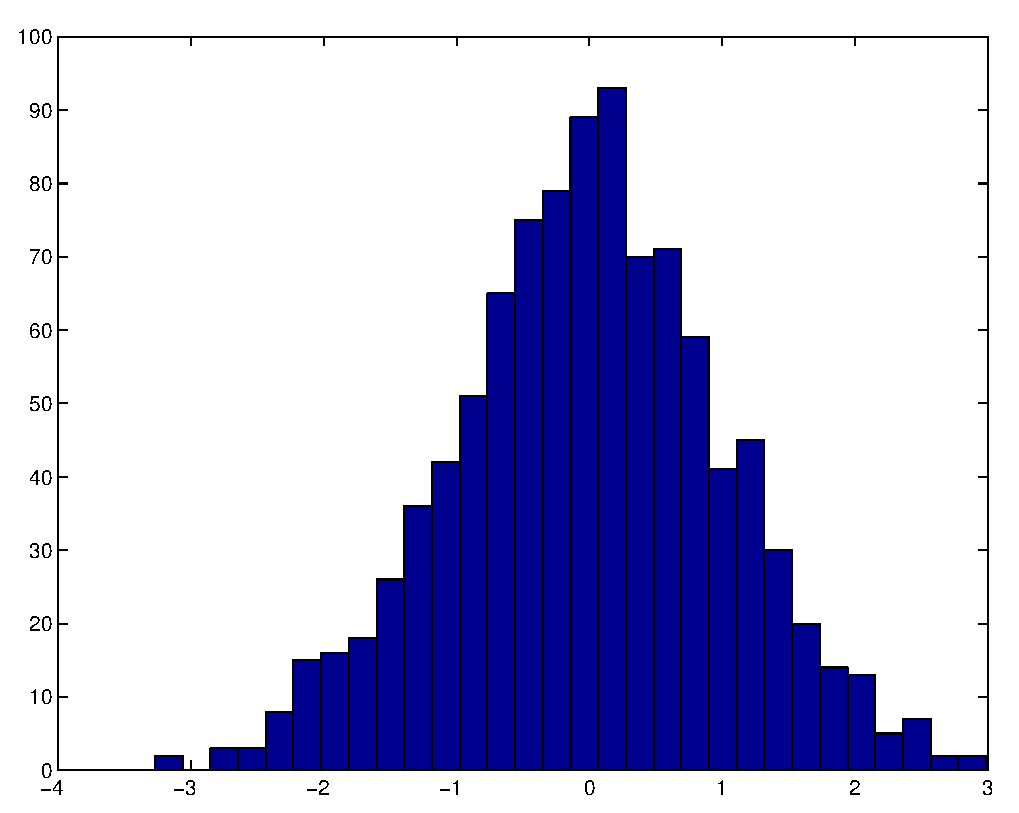
\includegraphics[width = 4.5 in ]{figure.eps}
\caption{Caption of a figure.}\label{FigureLabel}
\end{figure}

\begin{table}[h]
\centering \caption{The values of test
statistics and the corresponding critical values
at~$t_0.$~~$\alpha=0.1.$~}\label{stanford}\vskip .1in
\begin{tabular}{|c|c|c|c|c|c|c|}\hline
$t_0$ & 30 & 60 & 90 & 120 & 150 & 180 \\ \hline
Critical Value & 11.2282 & 10.5357 & 11.1108 & 11.7942 & 11.7343 & 11.7471\\ \hline
Test Statistic & 25.3182 & 24.6395 & 24.6049 & 25.6623 & 27.1320 & 29.3247\\ \hline
\end{tabular}
\end{table}

Here is how you cite an article, \cite{forina1991class}.